\section{Algorithm} \label{sec:algo}

The basic idea of the algorithm is similar to the one given in \cite{sano-sato:2020}: if $F$ is a field, $R$ is a multivariate polynomial ring over $F$, and $C$ is a freely and finitely generated chain complex over $R$ whose differential is homogeneous with respect to the polynomial grading, we may regard $C$ as a chain complex over $F$ and decompose it into (infinitely many) finitely generated subcomplexes. Having proved that these subcomplexes are acyclic except for finitely many ones, it follows that $H(C)$ can be fully computed algorithmically. For the reduced HOMFLY homology, the key to proving the finiteness is the symmetry (\Cref{prop:q-sym}).

Throughout this section, let $D$ be a non-trivial, connected, oriented link diagram with $n$ crossings. 

\subsection{Free variables of the edge ring}

\begin{lemma}[{\cite[Lemma 2.4]{Ras15}}]\label{dimlem}
    The reduced edge ring $R(D) = R'(D)/I(D)$ is isomorphic to a polynomial ring with $n$ variables.
\end{lemma}

\begin{proof}
    $R'(D)$ is generated by $2n$ indeterminates. The ideal $I(D)$ is generated by $1+n$ linear polynomials, and they have a unique linear relation $\sum_p \rho_p = 0$ since we assumed that $D$ is connected.
\end{proof}

\begin{figure}
    \centering
    

\tikzset{every picture/.style={line width=0.75pt}} %set default line width to 0.75pt        

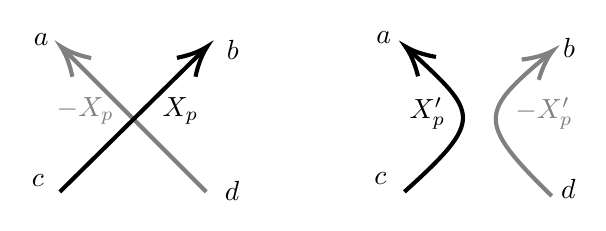
\begin{tikzpicture}[x=0.75pt,y=0.75pt,yscale=-1,xscale=1]
%uncomment if require: \path (0,109); %set diagram left start at 0, and has height of 109

%Straight Lines [id:da7979059503936952] 
\draw [color={rgb, 255:red, 128; green, 128; blue, 128 }  ,draw opacity=1 ][line width=1.5]    (39.62,19.12) -- (107.5,87) ;
\draw [shift={(37.5,17)}, rotate = 45] [color={rgb, 255:red, 128; green, 128; blue, 128 }  ,draw opacity=1 ][line width=1.5]    (14.21,-6.37) .. controls (9.04,-2.99) and (4.3,-0.87) .. (0,0) .. controls (4.3,0.87) and (9.04,2.99) .. (14.21,6.37)   ;
%Straight Lines [id:da7279842833116223] 
\draw [color={rgb, 255:red, 0; green, 0; blue, 0 }  ,draw opacity=1 ][line width=1.5]    (105.86,19.11) -- (37,87) ;
\draw [shift={(108,17)}, rotate = 135.41] [color={rgb, 255:red, 0; green, 0; blue, 0 }  ,draw opacity=1 ][line width=1.5]    (14.21,-6.37) .. controls (9.04,-2.99) and (4.3,-0.87) .. (0,0) .. controls (4.3,0.87) and (9.04,2.99) .. (14.21,6.37)   ;
%Curve Lines [id:da5605408166706283] 
\draw [color={rgb, 255:red, 0; green, 0; blue, 0 }  ,draw opacity=1 ][line width=1.5]    (203,87) .. controls (242.2,51.72) and (238.18,49.09) .. (205.53,18.88) ;
\draw [shift={(203.5,17)}, rotate = 402.85] [color={rgb, 255:red, 0; green, 0; blue, 0 }  ,draw opacity=1 ][line width=1.5]    (14.21,-6.37) .. controls (9.04,-2.99) and (4.3,-0.87) .. (0,0) .. controls (4.3,0.87) and (9.04,2.99) .. (14.21,6.37)   ;
%Curve Lines [id:da8925010918239024] 
\draw [color={rgb, 255:red, 128; green, 128; blue, 128 }  ,draw opacity=1 ][line width=1.5]    (274,89) .. controls (236.76,52.74) and (239.86,48.17) .. (272.47,20.71) ;
\draw [shift={(274.5,19)}, rotate = 499.95] [color={rgb, 255:red, 128; green, 128; blue, 128 }  ,draw opacity=1 ][line width=1.5]    (14.21,-6.37) .. controls (9.04,-2.99) and (4.3,-0.87) .. (0,0) .. controls (4.3,0.87) and (9.04,2.99) .. (14.21,6.37)   ;

% Text Node
\draw (23,9.4) node [anchor=north west][inner sep=0.75pt]    {$a$};
% Text Node
\draw (116,12.4) node [anchor=north west][inner sep=0.75pt]    {$b$};
% Text Node
\draw (22,77.4) node [anchor=north west][inner sep=0.75pt]    {$c$};
% Text Node
\draw (115,80.4) node [anchor=north west][inner sep=0.75pt]    {$d$};
% Text Node
\draw (85,40) node [anchor=north west][inner sep=0.75pt]  [color={rgb, 255:red, 0; green, 0; blue, 0 }  ,opacity=1 ]  {$X_p$};
% Text Node
\draw (34,40) node [anchor=north west][inner sep=0.75pt]  [color={rgb, 255:red, 128; green, 128; blue, 128 }  ,opacity=1 ]  {$-X_p$};
% Text Node
\draw (188,8.4) node [anchor=north west][inner sep=0.75pt]    {$a$};
% Text Node
\draw (278,11.4) node [anchor=north west][inner sep=0.75pt]    {$b$};
% Text Node
\draw (187,76.4) node [anchor=north west][inner sep=0.75pt]    {$c$};
% Text Node
\draw (277,79.4) node [anchor=north west][inner sep=0.75pt]    {$d$};
% Text Node
\draw (204,40) node [anchor=north west][inner sep=0.75pt]  [color={rgb, 255:red, 0; green, 0; blue, 0 }  ,opacity=1 ]  {$X'_p$};
% Text Node
\draw (255,40) node [anchor=north west][inner sep=0.75pt]  [color={rgb, 255:red, 128; green, 128; blue, 128 }  ,opacity=1 ]  {$-X'_p$};


\end{tikzpicture}
    \caption{$X_{p}$ and $X'_{p}$}
    \label{fig:crossing}
\end{figure}

Next we show that a generating set of $R(D)$ can be given by considering a spanning tree of the Seifert graph of $D$.
For each crossing $p$ of $D$, we define $X_{p}, X'_{p} \in R(D)$ by
\begin{align*}
    X_p &= x_b - x_c = -(x_a - x_d), \\
    X'_p &= x_a - x_c = -(x_b - x_d),
\end{align*}
where $a, b$ are outgoing edges at $p$ and $c,d$ are incoming edges at $p$, and $a, c$ are placed to the left of $p$ (see \Cref{complex,fig:crossing}).

\begin{lemma}[\cite{Nak20}]\label{treebasislem}
    Let $T$ be a spanning tree of the Seifert graph of $D$, and $S$ the set of crossings in $D$ corresponding to the edges of $T$.
    Then, $\mathcal{X}_T = \{X_p\}_{p \in S} \cup \{X'_p\}_{p \notin S}$ is an algebraically independent generating set of $R(D)$.
\end{lemma}

\begin{figure}
    \centering
    \tikzset{every picture/.style={line width=0.75pt}} %set default line width to 0.75pt        

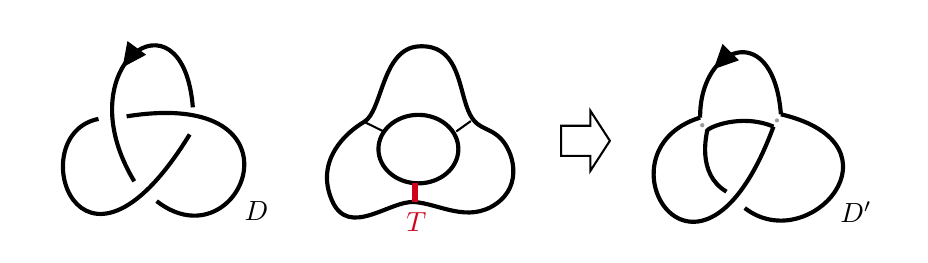
\begin{tikzpicture}[x=0.75pt,y=0.75pt,yscale=-1,xscale=1]
%uncomment if require: \path (0,109); %set diagram left start at 0, and has height of 109

\clip (0,0) rectangle (420,100);

%Curve Lines [id:da8161601596307948] 
\draw [line width=1.5]    (79.58,38.39) .. controls (74.8,-21.4) and (17.36,17.84) .. (51.36,74.01) ;
\draw [shift={(45.72,19.12)}, rotate = 306.15999999999997] [fill={rgb, 255:red, 0; green, 0; blue, 0 }  ][line width=0.08]  [draw opacity=0] (11.61,-5.58) -- (0,0) -- (11.61,5.58) -- cycle    ;
%Curve Lines [id:da5647400415250446] 
\draw [line width=1.5]    (62.15,83.58) .. controls (102.85,115.24) and (138.02,28.21) .. (47.66,42.73) ;
%Curve Lines [id:da13846906868786935] 
\draw [line width=1.5]    (34.13,43.95) .. controls (-3.3,51.35) and (24.68,138.29) .. (78.06,51.44) ;
%Curve Lines [id:da237486702787586] 
\draw [line width=1.5]    (362.91,41.73) .. controls (362.73,39.45) and (362.47,37.31) .. (362.15,35.31) .. controls (356.65,1.83) and (331.88,7.57) .. (325.49,31.04) .. controls (324.49,34.73) and (323.94,38.84) .. (323.99,43.32) ;
%Curve Lines [id:da6079162773576449] 
\draw [line width=1.5]    (345.48,86.91) .. controls (376.67,111) and (424.67,56.33) .. (362.91,41.73) ;
%Curve Lines [id:da012895447238909785] 
\draw [line width=1.5]    (323.99,43.32) .. controls (271.33,59.67) and (323.33,145) .. (359.33,47.67) ;
%Curve Lines [id:da4889524635526027] 
\draw [line width=1.5]    (359.33,47.67) .. controls (343.33,41) and (327.33,48.33) .. (327.33,49.67) .. controls (327.33,51) and (322,70.33) .. (336.67,79) ;
%Flowchart: Connector [id:dp9085114377251573] 
\draw  [draw opacity=0][fill={rgb, 255:red, 155; green, 155; blue, 155 }  ,fill opacity=1 ] (323.97,46.98) .. controls (323.97,46.42) and (324.43,45.96) .. (324.99,45.96) .. controls (325.55,45.96) and (326.01,46.42) .. (326.01,46.98) .. controls (326.01,47.54) and (325.55,48) .. (324.99,48) .. controls (324.43,48) and (323.97,47.54) .. (323.97,46.98) -- cycle ;
%Flowchart: Connector [id:dp9045304281632592] 
\draw  [draw opacity=0][fill={rgb, 255:red, 155; green, 155; blue, 155 }  ,fill opacity=1 ] (360,44.67) .. controls (360,44.11) and (360.45,43.67) .. (361,43.67) .. controls (361.55,43.67) and (362,44.11) .. (362,44.67) .. controls (362,45.22) and (361.55,45.67) .. (361,45.67) .. controls (360.45,45.67) and (360,45.22) .. (360,44.67) -- cycle ;
%Shape: Polygon Curved [id:ds49799004625007537] 
\draw  [line width=1.5]  (162.13,45.37) .. controls (171.07,40.12) and (170.5,10) .. (188.5,9) .. controls (206.5,8) and (207.42,26.18) .. (211.5,38) .. controls (215.58,49.82) and (221.05,46.9) .. (227.5,53) .. controls (233.95,59.1) and (238.94,75.83) .. (225.5,85) .. controls (212.06,94.17) and (198.5,85) .. (186.5,84) .. controls (174.5,83) and (154.5,102) .. (146.5,83) .. controls (138.5,64) and (153.18,50.62) .. (162.13,45.37) -- cycle ;
%Shape: Ellipse [id:dp8656777374199306] 
\draw  [line width=1.5]  (169,58.5) .. controls (169,49.39) and (177.62,42) .. (188.25,42) .. controls (198.88,42) and (207.5,49.39) .. (207.5,58.5) .. controls (207.5,67.61) and (198.88,75) .. (188.25,75) .. controls (177.62,75) and (169,67.61) .. (169,58.5) -- cycle ;
%Straight Lines [id:da1480688684375554] 
\draw    (162.13,45.37) -- (171.5,50) ;
%Straight Lines [id:da3873077880987402] 
\draw    (213.5,45) -- (206.5,50) ;
%Straight Lines [id:da043234858474899274] 
\draw [color={rgb, 255:red, 208; green, 2; blue, 27 }  ,draw opacity=1 ][line width=2.25]    (186.5,75) -- (186.5,84) ;
%Straight Lines [id:da23585575290034488] 
\draw [line width=1.5]    (335.5,15) -- (333.33,17.17) ;
\draw [shift={(330.5,20)}, rotate = 315] [fill={rgb, 255:red, 0; green, 0; blue, 0 }  ][line width=0.08]  [draw opacity=0] (11.61,-5.58) -- (0,0) -- (11.61,5.58) -- cycle    ;
%Right Arrow [id:dp28729390632428686] 
\draw   (257,47.25) -- (271.1,47.25) -- (271.1,40) -- (280.5,54.5) -- (271.1,69) -- (271.1,61.75) -- (257,61.75) -- cycle ;

% Text Node
\draw (103,82.4) node [anchor=north west][inner sep=0.75pt]    {$D$};
% Text Node
\draw (390,82.4) node [anchor=north west][inner sep=0.75pt]    {$D'$};
% Text Node
\draw (181,87.4) node [anchor=north west][inner sep=0.75pt]    {$\textcolor[rgb]{0.82,0.01,0.11}{T}$};


\end{tikzpicture}
    \caption{$D, T$ and $D'$}
    \label{fig:treebasislem}
\end{figure}

\begin{proof}
    Working over $\QQ$ allows us to have the equation
    \[
    \QQ[x_1, \ldots , x_m] = \QQ[x_1-x_2,\ x_2-x_3,\ \ldots,\ x_{m-1}-x_m,\ x_1+\cdots+x_m].
    \]
    Thus it follows that $R(D)$ is generated by elements of the form $x_e - x_f$, where $e, f$ are edges of $G(D)$.
    Since $|\mathcal{X}_T| = n$, it is enough to show that each $x_e - x_f$ can be written as a linear sum of elements in $\mathcal{X}_T$.
    Since $D$ is connected, by resolving all crossings in $D$ which are not in $S$, we obtain a diagram $D'$ of the trivial knot (see \Cref{fig:treebasislem} for an easy case).
    There is a unique oriented path $\gamma$ in $G(D')$ from $f$ to $e$, which may be also regarded as a path in $G(D)$.
    Trace $\gamma$ from $x_f$ to $x_e$, and each time $\gamma$ passes a crossing $p$ in $D$, take a term $\pm X_p$ or $\pm X'_p$ according to how $\gamma$ passes $p$ (see \Cref{fig:crossing}).
    It is obvious that these terms belong to $\mathcal{X}_T$ and that the sum gives $x_e-x_f$.
\end{proof}

\subsection{Reinterpretation as cube complexes} \label{subsec:double-cube-cpx}

Next we reinterpret the chain complex $C(D)$ given in \Cref{sec:prelim} as a ``double cube complex". Precise statement follows.

The \textit{$n$-cube} is a poset $\{0, 1\}^n$ with the product order of $0 < 1$, considered as a category.
An object $v \in \{0, 1\}^n$ is called a \textit{vertex}, and the Manhattan norm of $v$ is denoted by $|v| = v_1 + \cdots + v_n$. A morphism $v \to w$ such that $|v| + 1 = |w|$ is denoted $v \to_1 w$ and called an \textit{edge}. Define vertices $\bar{0} = (0, \ldots, 0)$ and $\bar{1} = (1, \ldots, 1)$.

\begin{figure}
    \centering
    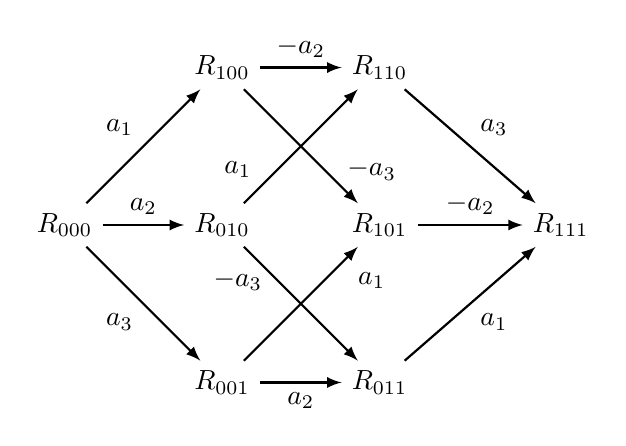
\begin{tikzpicture}[auto]
    \node (v0) at (-3.5,0.5) {$R_{000}$};
    \node (v1) at (-1.5,2.5) {$R_{100}$};
    \node (v2) at (-1.5,0.5) {$R_{010}$};
    \node (v3) at (-1.5,-1.5) {$R_{001}$};
    \node (v4) at (0.5,2.5) {$R_{110}$};
    \node (v5) at (0.5,0.5) {$R_{101}$};
    \node (v6) at (0.5,-1.5) {$R_{011}$};
    \node (v7) at (2.8,0.5) {$R_{111}$};
    \draw[-latex, thick] (v0) to node {$a_1$} (v1);
    \draw[-latex, thick] (v0) to node {$a_2$} (v2);
    \draw[-latex, thick] (v0) to node[swap] {$a_3$} (v3);
    \draw[-latex, thick] (v1) to node {$-a_2$} (v4);
    \draw[-latex, thick] (v1) edge (v5);
    \draw[-latex, thick] (v2) edge (v4);
    \draw[-latex, thick] (v2) edge (v6);
    \draw[-latex, thick] (v3) edge (v5);
    \draw[-latex, thick] (v3) to node[swap] {$a_2$} (v6);
    \draw[-latex, thick] (v4) to node {$a_3$} (v7);
    \draw[-latex, thick] (v5) to node {$-a_2$} (v7);
    \draw[-latex, thick] (v6) to node[swap] {$a_1$} (v7);
    \node at (0.4,-0.2) {$a_1$};
    \node at (0.4,1.2) {$-a_3$};
    \node at (-1.3,-0.2) {$-a_3$};
    \node at (-1.3,1.2) {$a_1$};
\end{tikzpicture}

    \caption{A cube complex with factors $(a_1, \ldots, a_n)$.}
    \label{fig:cube-complex}
\end{figure}

Let $\mathcal{A}$ be an additive category.
\begin{definition}
    For $n \geq 0$, an \textit{$n$-cube in $\mathcal{A}$} is a functor $\mathcal{C}\colon \{0, 1\}^n \to \mathcal{A}$.
\end{definition}

Given an $n$-cube $\mathcal{C}$ in $\mathcal{A}$,
one obtains a \textit{cube complex} $(C^*, d^*)$ in $\mathcal{A}$ with 
\[
    C^i = \bigoplus_{|v| = i} \mathcal{C}(v)
\]
and differentials
\[
    d^i = \sum_{\substack{|v| = i,\\ e\colon v \to w}} s(e)\mathcal{C}(e),
\]
by choosing $s(e) \in \{\pm 1\}$ for each edge $e$ of the cube so that for any square consisting of four edges $e_1,\ldots,e_4$, we have $s(e_1) \cdots s(e_4) = -1$.

\begin{remark}
    The isomorphism class of the above cube complex is independent of the choice of $s$.
\end{remark}

Now we put $C(D)$ in this framework. First we will ignore the original homological gradings, and lately relate them with the newly introduced gradings. 
%
We recall that $C(D)$ is a tensor product of (vertical) two-terms complexes of (horizontal) complexes. Hence $C(D)$ can be regarded as a cube complex of complexes. We write 
\[
    C(D) = \bigoplus_{v \in \{0, 1\}^n} C^*_v(D),
\]
where $C^*_v(D)$ is the complex at a vertex $v \in \{0, 1\}^n$, called the \textit{horizontal complex} of $D$ at $v$.
Since $C^*_v(D)$ is also a tensor product of two-terms complex over $R(D)$, it can be regarded as a cube complex again. We write
\[
    C^*_v(D) = \bigoplus_{h \in \{0, 1\}^n} R_{v, h}(D),
\]
where $R_{v, h}(D)$ is the module at a vertex $h \in \{0, 1\}^n$, and it is indeed a shifted copy of $R(D)$. The horizontal differential 
\[
    d_H: C^*_v(D) \rightarrow C^{*+1}_v(D)
\]
has the following form.
For each standard unit vector $e_i$ of $\RR^n$, there exists an element $a_i$ of $R(D)$ such that for any edge $v \to_1 w$ in the direction of $e_i$ in the $n$-cube, the corresponding map $R_{v,h}(D) \to R_{w,h}(D)$ summed in $d_H$ is the multiplication map by $a_i$ as specified by the horizontal arrows of \Cref{complex} according to $v$ (with some appropriate sign assignment). We call $a_1, \ldots, a_n$ the \textit{factors} of $C^*_v(D)$ (see \Cref{fig:cube-complex}).

By taking the homology with respect to $d_H$, we get a cube complex of homologies
\[
    \bigoplus_{v \in \{0, 1\}^n} H^*(C_v(D), d_H)
\]
with differential $(d_V)_*$. Then it is obvious that $\Hhat(D)$ is given by the homology of this complex
\[
    \Hhat(D) = H(\oplus_v (H(C_v(D), d_H), (d_V)_*).
\]

The homological bigrading $(\alpha, \beta)$ of the double cube complex $C(D)$ correspond to the original bigrading $(j, k)$ as
\[
    (\alpha, \beta) = \frac{1}{2}(j - j_0,\ k - k_0)
\]
where $(j_0, k_0)$ is the (original) homological bidegree of the module $R_{\bar{0}, \bar{0}}(D)$ placed at $(v, h) = (\bar{0}, \bar{0})$. For later use, let $i_0$ denote the $q$-grading shift of $R_{\bar{0}, \bar{0}}(D)$. Then from \Cref{complex} we have 
%
\begin{equation} \label{eq:ijk0}
    (i_0, j_0, k_0) = (2n^+, -2n, -2n^+)
\end{equation}
%
where $n_+$ and $n_-$ are the number of positive and negative crossings of $D$ respectively.

\subsection{Slicing by $q$-degrees} 

As described in \Cref{treebasislem}, the ring $R(D)$ can be represented by a multivariate polynomial ring $\QQ[X_i]$ with $n$ variables, so we have a homogeneous decomposition of $R(D)$ as a $\QQ$-vector space
\[
    R(D) \isom \QQ(1) \oplus \QQ(X_i)_{1 \leq i \leq n}  \oplus \QQ(X_i X_j)_{1 \leq i \leq j \leq n} \cdots.
\]
Let $i_{v, h} \in \ZZ$ be the $q$-grading shift of $R_{v, h}(D) = R(D)\{i_{v, h}\}$. Decompose $R_{v, h}(D)$ as 
\[
    R_{v, h}(D) = \bigoplus_{l = -\infty}^\infty V_{l, v, h}(D)
\]
so that each $V_{l, v, h}(D)$ is homogeneous of $q$-degree $2(l + |h|) + i_0$. It is generated by monomials 
% $X_{i_1} \cdots X_{i_e}$ 
of degree (in the usual sense) 
%
\begin{equation} \label{eq:monomial-degree}
    e(l, v, h) = l + |h| + \frac{i_0 - i_{v, h}}{2}.
\end{equation}
%
Now define 
\[
    C_l(D) = \bigoplus_{v, h} V_{l, v, h}(D)
\]
then it is obvious that both $d_H, d_V$ are closed in $C_l(D)$.  Regarding $C(D)$ as a chain complex over $\QQ$, we get a decomposition
\[
    C(D) = \bigoplus_{l = -\infty}^\infty C_l(D).
\]
We call each subcomplex $C_l(D)$ the \textit{level-$l$ slice} of $C(D)$. Note that the decomposition is defined so that $V_{l, \bar{0}, \bar{0}}(D)$ is generated by monomials of degree $e = l$. 

\begin{lemma}
    $C_l(D) = 0$ for $l < -2n$.
\end{lemma}

\begin{proof}
    The claim is clear since $e$ is non-decreasing with respect to $v, h$ and $e(l, \bar{1}, \bar{1}) = l + 2n$.
\end{proof}

From the previous arguments, it is obvious that each $C_l(D)$ may also be regarded as a double cube complex. Define the \textit{level-$l$ slice} $C_{l, v}(D)$ of the horizontal complex $C_v(D)$ at $v \in \{0, 1\}^n$ by
\[
    C_{l, v}(D) = \bigoplus_{h \in \{0, 1\}^n} V_{l, v, h}(D).
\]
Then we get a decomposition
\[
    \Hhat(D) = \bigoplus_{l = -2n}^\infty \Hhat_l(D),
\]
where 
\[
    \Hhat_l(D) = H(\oplus_v (H(C^*_{l, v}(D), d_H), (d_V)_*).
\]

We claim that each $\Hhat_l(D)$ is algorithmically computable. To take the homology twice, we find a basis on each chain group $C^i = C^i_{l, v}(D)$ that gives a decomposition
\[
    C^i = H^i \oplus B^i \oplus (d^i_H)^{-1}(B^{i + 1})
\]
so that we get representative cycles of the generators of $H^i = H^i(C^*_{l, v}(D))$ and that the secondary homology computation can be done on the chain level. This is achieved by standard methods such as the Gaussian elimination. 

\begin{proposition}
    For a link diagram $D$, the homology $\Hhat(D)$ has a decomposition
    \[
        \Hhat(D) = \bigoplus_{l = -2n}^{\infty} \Hhat_l(D)
    \]
    where each summand $\Hhat_l(D)$ can be computed algorithmically. Moreover for each triple degree $(i, j, k)$ we have 
    %
    \begin{equation} \label{eq:Hijk}
        \Hhat^{i, j, k}(D) = H^\beta(\oplus_v (H^\alpha(C^*_{v, l}(D), d_H), (d_V)_*)
    \end{equation}
    %
    where
    %
    \[
        (l, \alpha, \beta) = \frac{1}{2}((i - i_0) - (j - j_0),\ j - j_0,\ k - k_0)
    \]
    and $(i_0, j_0, k_0)$ are given as in \eqref{eq:ijk0}. Similar statement holds for $\Hbar(D)$. \qed
\end{proposition}

Now we restrict to the case where $D$ is a knot diagram, and in particular where it is a braid closure. In such case, it is well-known that $\Hbar(D)$ is finite dimensional \cite{Ras15}. In order to perform the actual calculation, we must specify an actual upper bound for the level $l$.

\begin{proposition} \label{prop:finiteness}
    If $K$ is a knot with braid closure diagram $D$, then
    \[
        \Hbar(K) \isom \bigoplus_{l = -2n}^{-n} \Hbar_l(D).
    \]
    Moreover, $\Hbar(K)$ can be obtained from the computations of $\Hbar^{i, j, k}(D)$ within the following ranges:
    \begin{align*}
        i &\in [-n + s - 1, 0], \tag{1}\\
        j &\in [w - s + 1, w + s - 1], \tag{2}\\
        k,\ k + 2i &\in [-n + s - 1, n - s + 1]. \tag{3}
    \end{align*}
\end{proposition}

\begin{proof}
    From \Cref{prop:MFW-ineq,prop:morton} and equation \eqref{eq:Hbar-def}, it follows that $\Hbar_l(D)$ is supported in 
    \begin{align*}
        2l 
        &= (i - i_0) - (j - j_0) \\ 
        &\leq \{ (n - s + 1) - (-w + s - 1) - 2n^+ \}\\
        &\quad - \{(w - s + 1) - (w + s - 1) - (-2n)\}\\
        &= -2n.
    \end{align*}
    For the latter statement: (1) the lower bound is given by the Morton bound (\Cref{prop:morton}), and from \Cref{prop:q-sym} it suffices to compute $H^{i, *, *}(D)$ within $i \leq 0$.
    (2) This is exactly \Cref{prop:MFW-ineq}.
    (3) The lower bound of $k$ is obvious from the definition of $C(D)$, and from \Cref{prop:duality} we also have the upper bound. From \Cref{prop:q-sym}, $k + 2i$ must also lie in this range.
\end{proof}

\subsection{Exclusion of variables}

As apparent from \eqref{eq:monomial-degree}, the number of generators increases combinatorially as $l$ increases. In order to reduce the computational cost, we use the process called ``exclusion of variables" as described in \cite[Lemma 3.8]{Ras15}. 

Again we assume $D$ is a link diagram. Put $R = R(D)$. Take any $v \in \{0, 1\}^n$ and consider the horizontal cube complex $C = C_v(D)$. Take any factor $f \in R$ of $C$. Note that $f$ is either linear or quadratic.

After choosing an appropriate sign assignment, $C$ may be regarded as the mapping cone of the endomorphism 
\[
    C' \xrightarrow{f} C'
\]
of an $n-1$ dimensional cube complex $C'$. Let $d, d'$ denote the differentials of $C, C'$ respectively. The complex $C$ is isomorphic to $C' \oplus C'$ as an $R$-module, and we can write
\[
    d(x_0, x_1) = (-d'x_0, fx_0 + d'x_1).
\]

Now $f$ is monic with respect to some variable $X_k$. Define
\[
R_0 = \QQ[X_1, \ldots \widehat{X_k}, \ldots, X_n].
\]
Let $\pi \colon R \rightarrow R_1 = R/(f)$ be the quotient map, $\iota \colon R_1 \rightarrow R$ be the map that sends any residue class $[g] \in R_1$ to the remainder of $g$ by $f$ with respect to the variable $X_k$.
We note that $\pi$ and $\iota$ are homomorphisms of modules over $R$ and $R_0$ respectively.
Let $C'' = C' \otimes_R R_1$, and let $d''$ be the differential of $C''$. Two chain maps $\phi \colon C \rightarrow C''$ and $\psi \colon C'' \rightarrow C$ over $R_0$ are given by
\[
    \phi(x_0, x_1) = \pi(x_1),
\]
and
\[
    \psi(y) = \left(\frac{\iota(d''y) - d'\iota(y)}{f},\  \iota(y)\right),
\]
and it is not hard to verify that $\psi \phi \htpy \id_C$ and $\phi \psi = \id_{C''}$.
The complex $C''$ admits the obvious triple grading so that both $\phi, \psi$ are degree preserving. Thus the two maps restrict as chain homotopy equivalences between the two sliced complexes $C_l$ and $C''_l$. The effect is that $H(C_l) \cong H(C''_l)$ can be computed with fewer generators, which is drastic when $l$ becomes large. 

Furthermore, this process of reduction can be repeated for other directions as long as the target variable is algebraically independent in the base ring. When $f$ is linear, we have $R_1 \isom R_0$ and all other variables remain independent. When $f$ is quadratic, then $R_1 \isom R_0 \otimes_\QQ \QQ\{1, X_k\}$ as $\QQ$-vector spaces, and the variables that does not appear in the coefficients of $f$ remains independent.

In particular, when all factors $f$ of $C$ are linear, then the exclusion can be continued until the differential becomes trivial. In general, to exclude the variables as much as possible, it is preferable to perform exclusions on linear polynomials first, and then on the remaining quadratics. 

For the computation of $\Hbar(D)$, we can replace each horizontal complex $C_{l, v}$ with a reduced one, compute those homologies, and replace the differential $(d_V)_*$ on the vertical complex with $(\phi_{v'} \circ d_V \circ \psi_v)_*$ for each edge $v \rightarrow v'$. 

\subsection{Overall procedure}

We summarize the overall procedure for computing (the dimensions of) the reduced HOMFLY homology $h^{i, j, k} = \{\dim \Hbar^{i, j, k}(K)\}_{i, j, k}$ of a knot $K$.

\begin{algorithm}\label{algo:basic}
    Given a braid closure diagram $D$ of a knot $K$, 
    \begin{enumerate}
        \item Compute the Seifert graph $G(D)$ and find a spanning tree $T$ of $G(D)$. 
        
        \item Using $T$, identify the edge ring $R(D)$ as a multivariate polynomial ring, and represent both $d_H$ and $d_V$ as $n$-tuples of polynomials in $R(D)$ as in the proof of \Cref{treebasislem}.
        
        \item For each $(l, \alpha, \beta)$ in $[-2n, -n] \times [0, n] \times [0, n]$:
        \begin{enumerate}
            \item Convert $(l, \alpha, \beta)$ to $(i, j, k)$. Skip to the next iteration if $(i, j, k)$ is not in the range of \Cref{prop:finiteness}.
            
            \item Setup the generators of the level-$l$ horizontal complex $C_l(D)$.
            
            \item Perform exclusion of variables on $C_l(D)$ to get a reduced complex together with the chain homotopy equivalences. 

            \item Compute $h^{i, j, k} = \dim \Hbar^{i, j, k}(D)$ from \eqref{eq:Hijk}, with the horizontal complexes replaced with the reduced ones. 
            
            \item Assign $h^{-i, j, k + 2i} = h^{i, j, k}$ if $i < 0$.
        \end{enumerate}
        \item Return $h$.
    \end{enumerate}
\end{algorithm}

Reusable data should be cached within the iteration. Further improvement can achieved by concerning mirrors of knots. To explain this, assume that $D$ has only one crossing $p$. Recall that the vertex module $V_{l, v, h}(D)$ at $(v, h) \in \{0, 1\}^2$ is spanned by the monomials of degree given  by \eqref{eq:monomial-degree}. From \Cref{complex}, we see that $e(l, 1, 0) = e(l, 0, 1) = e(l, 0, 0) + 1$ if $p$ is positive, and $e(l, 1, 0) = e(l, 0, 1) = e(l, 0, 0)$ if $p$ is negative (in both cases $e(l, 1, 1) = e(l, 0, 0) + 1$). This means that $C_l(D)$ has a smaller generating set when $p$ is negative. In general if $w(D) > 0$, then $C_l(m(D))$ has a smaller generating set than $C_l(D)$. This difference becomes intense as $n$ increases. Thus the improved version is:

\begin{algorithm}\label{algo:mirror}
    Given a braid closure representative $D$ of a knot $K$, \begin{enumerate}
        \item If $w(D) \leq 0$, compute and return $h(D)$ by \Cref{algo:basic}.
        \item Otherwise, compute $h(m(D))$ by \Cref{algo:basic} and return its dual.
    \end{enumerate}
\end{algorithm}